\documentclass[serif, mathsansserif, aspectratio=169]{beamer}   % [handout] to remove pause

\setbeamertemplate{title page}[default][left]  % left-align title page
\beamertemplatenavigationsymbolsempty % remove navigation symbols

\usepackage{sourcesanspro}
\usepackage[T1]{fontenc}
\usepackage[utf8]{inputenc}
\usepackage[document]{ragged2e}
\usepackage{hyperref}
\usepackage{fontawesome5}
\usepackage[tracking=true]{microtype}
\usepackage[scaled=0.90]{helvet}
\usepackage[scaled=0.85]{beramono}
\usepackage{tgpagella}
\usepackage{mathpazo}
\usepackage{mathtools}
\usepackage{amsmath}
\usepackage{amssymb}
\usepackage{amsthm}
\usepackage{scalerel}
\usepackage{bm}
\usepackage{bbm}
\usepackage{xcolor}
\usepackage{enumerate}
\usepackage{soul}
\usepackage{tikz}
\usepackage{listings}
\usepackage{lstbayes}
\usepackage{booktabs}
\usepackage{bold-extra}
\usepackage{textpos}
\usepackage{multirow}
\usepackage{longtable}
\usepackage{tabularx}
\usepackage[flushleft]{threeparttable}
\usepackage{varwidth}

\usepackage{xpatch}
\usepackage[plain]{algorithm}
\usepackage{algorithmicx}
\usepackage[noend]{algpseudocode}

\usepackage{graphicx}
\usepackage{fancybox}


\usepackage[skins,theorems]{tcolorbox}
\tcbset{highlight math style={enhanced,colframe=red,colback=white,arc=0pt,boxrule=1pt}}

%%%%%%%%%%%%%%%%%%%%%%%%%%%%%%%%%%%%%%%%%%%%%%%%%%
% Bibliography settings
%%%%%%%%%%%%%%%%%%%%%%%%%%%%%%%%%%%%%%%%%%%%%%%%%%
\usepackage[backend=biber, style=apa, autocite=inline, doi=false, url=false]{biblatex}
\DeclareLanguageMapping{english}{english-apa}
\setcounter{biburlnumpenalty}{85}  % for urls that are too long
\addbibresource{bibliography.bib}
\setbeamertemplate{bibliography item}{}% Remove reference icon.
\setbeamercolor{bibliography entry author}{fg=bonnblue}
\setbeamercolor{bibliography entry note}{fg=bonnblue}
\renewcommand*{\bibfont}{\footnotesize}
\AtEveryBibitem{%
  \clearfield{volume}%
  \clearfield{number}%
  \clearfield{pages}%
}


%%%%%%%%%%%%%%%%%%%%%%%%%%%%%%%%%%%%%%%%%%%%%%%%%%
% Algorithm
%%%%%%%%%%%%%%%%%%%%%%%%%%%%%%%%%%%%%%%%%%%%%%%%%%
\makeatletter
\xpatchcmd{\algorithmic}{\itemsep\z@}{\itemsep=1ex plus1pt}{}{}
\makeatother



%%%%%%%%%%%%%%%%%%%%%%%%%%%%%%%%%%%%%%%%%%%%%%%%%%
% Math definitions
%%%%%%%%%%%%%%%%%%%%%%%%%%%%%%%%%%%%%%%%%%%%%%%%%%
\newcommand\indicator[1]{\scaleobj{1.4}{\mathbbm{1}} \! \left\{#1\right\}}
\newcommand\expectation[1]{\mathbb{E}\left[#1\right]}

\DeclareMathOperator*{\argmax}{argmax}


%%%%%%%%%%%%%%%%%%%%%%%%%%%%%%%%%%%%%%%%%%%%%%%%%%
% Colors
%%%%%%%%%%%%%%%%%%%%%%%%%%%%%%%%%%%%%%%%%%%%%%%%%%
\definecolor{bonnblue}{RGB}{4, 83, 156}  % hex: #04539C
\definecolor{bonngrey}{RGB}{148, 147, 132}  % hex: #8A9384
\definecolor{bonnyellow}{RGB}{251, 187, 6}  % hex: #FBBB06
\definecolor{red}{RGB}{65, 16, 16}  % hex: #411010

%%%%%%%%%%%%%%%%%%%%%%%%%%%%%%%%%%%%%%%%%%%%%%%%%%
% Auxiliary files
%%%%%%%%%%%%%%%%%%%%%%%%%%%%%%%%%%%%%%%%%%%%%%%%%%
\newcommand{\email}[1]{\def\@email{\texttt{\MakeLowercase{\textls[10]{#1}}}}}

\setbeamerfont{title}{series=\bfseries} % family=\sourcesanspro
\setbeamerfont{subtitle}{series=\scshape, size*={8}{15}} % family=\sourcesanspro
\setbeamercolor{subtitle}{fg=black}
\setbeamerfont{author}{family=\scshape}

\setbeamercolor{title}{fg=black}
\setbeamercolor{author}{fg=bonnblue}
\setbeamercolor{institute}{fg=bonngrey}
\setbeamercolor{email}{fg=bonnyellow}

\defbeamertemplate*{title page}{customized}[1][]
{
    \usebeamerfont{title}\usebeamercolor[fg]{title}\textls[100]{\MakeUppercase{\textbf{\inserttitle}}}\par
    \usebeamerfont{subtitle}\usebeamercolor[fg]{subtitle}\textls[100]{\textsc{\insertsubtitle}}\par\par
    \vfill
    \usebeamerfont{author}\usebeamercolor[fg]{author}\textls[100]{\textsc{\insertauthor}}\par
    \usebeamerfont{institute}{\usebeamercolor[fg]{institute}\textls[100]{\textsc{\insertinstitute}}}\par
    \bigskip
    {\usebeamercolor[fg]{email}\@email}\par
    \usebeamerfont{date}\insertdate\par
    \usebeamercolor[fg]{titlegraphic}\inserttitlegraphic
}



%%%%%%%%%%%%%%%%%%%%%%%%%%%%%%%%%%%%%%%%%%%%%%%%%%
% Auxiliary commands
%%%%%%%%%%%%%%%%%%%%%%%%%%%%%%%%%%%%%%%%%%%%%%%%%%
% \graphicspath{files/} % graphics path
\newcommand{\labelitem}{\tikz\draw[black,fill=bonnblue] (0,0) circle (.35ex); \,\,}

\newcommand{\blue}[1]{\textcolor{bonnblue}{#1}}
\newcommand{\yellow}[1]{\textcolor{bonnyellow}{#1}}
\newcommand{\grey}[1]{\textcolor{bonngrey}{#1}}
\newcommand{\red}[1]{\textcolor{red}{#1}}


%%%%%%%%%%%%%%%%%%%%%%%%%%%%%%%%%%%%%%%%%%%%%%%%%%
% Beamer settings
%%%%%%%%%%%%%%%%%%%%%%%%%%%%%%%%%%%%%%%%%%%%%%%%%%
\setbeamercolor{itemize item}{fg=black}
\setbeamercolor{itemize subitem}{fg=black}
\setbeamercolor{itemize subsubitem}{fg=black}
\setbeamercolor{section head}{fg=cardinal} % currently unused.
\setbeamercolor{footline}{fg=bonnblue}
\setbeamercolor{section in toc}{fg=black}

\setbeamertemplate{itemize item}[circle]
\setbeamertemplate{itemize subitem}{{\textendash}}
\setbeamertemplate{itemize subsubitem}[triangle]
\setbeamertemplate{section in toc}{{\inserttocsectionnumber.}~\inserttocsection}

\setbeamerfont{section in toc}{series=\scshape, size=\Large}
\setbeamerfont{frametitle}{series=\scshape} % \itshape
\setbeamercolor{frametitle}{fg=bonnblue}

\setbeamertemplate{frametitle}
{
    \vspace*{0.4cm}
    \insertframetitle \\ \footnotesize \textcolor{bonngrey}{\insertframesubtitle}
}

\AtBeginSection[]{
  \setbeamertemplate{footline}[frame number]{}
  \setbeamertemplate{navigation symbols}{}
  \setbeamertemplate{footline}{}
  \begin{frame}
  \vfill
  \centering
  \begin{beamercolorbox}[sep=8pt,center]{title}
    {\usebeamerfont{title}\usebeamercolor[fg]{title}{\textsc{\insertsectionhead}}}\par%
  \end{beamercolorbox}
  \vfill
  \end{frame}
  \addtobeamertemplate{navigation symbols}{}{%
      \usebeamerfont{footline}%
      \usebeamercolor[fg]{author}%
      \hspace{1em}%
      \raisebox{1em}[0pt][0pt]{%
      \small \insertframenumber/\inserttotalframenumber \kern 0.25em
      }
  }
}

\AtBeginSubsection[]{
  \setbeamertemplate{footline}[frame number]{}
  \setbeamertemplate{navigation symbols}{}
  \setbeamertemplate{footline}{}
  \begin{frame}
  \vfill
  \centering
  \begin{beamercolorbox}[sep=8pt,center]{title}
      {\usebeamerfont{title}\usebeamercolor[fg]{title}{\textsc{{\normalsize
      \grey{\insertsectionhead}}\\[1em] \insertsubsectionhead}}}\par%
  \end{beamercolorbox}
  \vfill
  \end{frame}
  \addtobeamertemplate{navigation symbols}{}{%
      \usebeamerfont{footline}%
      \usebeamercolor[fg]{author}%
      \hspace{1em}%
      \raisebox{1em}[0pt][0pt]{%
      \small \insertframenumber/\inserttotalframenumber \kern 0.25em
      }
  }
}



\title{Topics in Econometrics and Statistics}
\subtitle{Summer term, 2021}
\author{Tim Mensinger}
\institute{University of Bonn}
\email{tmensinger@uni-bonn.de}
\date{}

% math color
% \makeatletter
% \def\mathcolor#1#{\@mathcolor{#1}}
% \def\@mathcolor#1#2#3{%
%   \protect\leavevmode
%   \begingroup
%     \color#1{#2}#3%
%   \endgroup
% }
% \makeatother

% algorithm numbering
%\makeatletter
%\renewcommand{\fnum@algorithm}{\fname@algorithm}
%\makeatother

% caption color
% \setbeamercolor{caption name}{fg=myred}

% settings frame body
% \setbeamerfont*{standout}{series=\bfseries, size=\huge}


\begin{document}


\begin{frame}
    \maketitle
\end{frame}

% Page numbers
\addtobeamertemplate{navigation symbols}{}{%
    \usebeamerfont{footline}%
    \usebeamercolor[fg]{author}%
    \hspace{1em}%
    \raisebox{1em}[0pt][0pt]{%
    \small \insertframenumber/\inserttotalframenumber \kern 0.25em
    }
}
\begin{frame}
  \tableofcontents
\end{frame}


\section{Introduction}


\subsection{Motivation}

\begin{frame}{Paper}{Liebl et al. (2020)}
\begin{figure}[ht]
    \centering
    \vspace{-0.8cm}
    \shadowbox{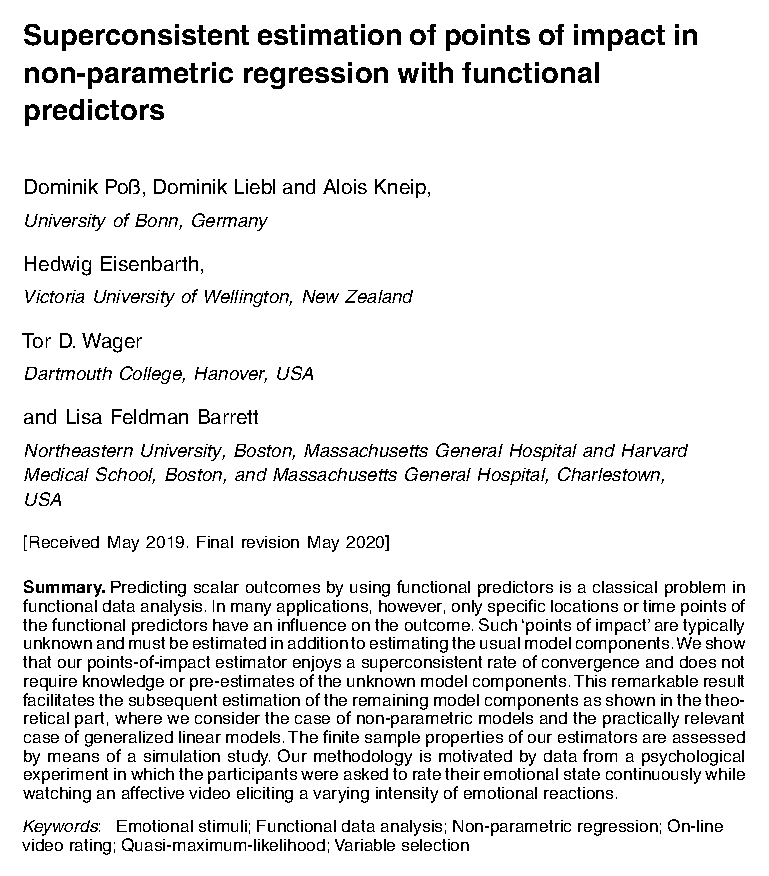
\includegraphics[width=0.45\textwidth]{files/paper-titlepage.pdf}}
\end{figure}
\end{frame}

\begin{frame}{The Setting}{Liebl et al. (2020)}
\begin{figure}[ht]
    \centering
    \vspace{-1cm}
    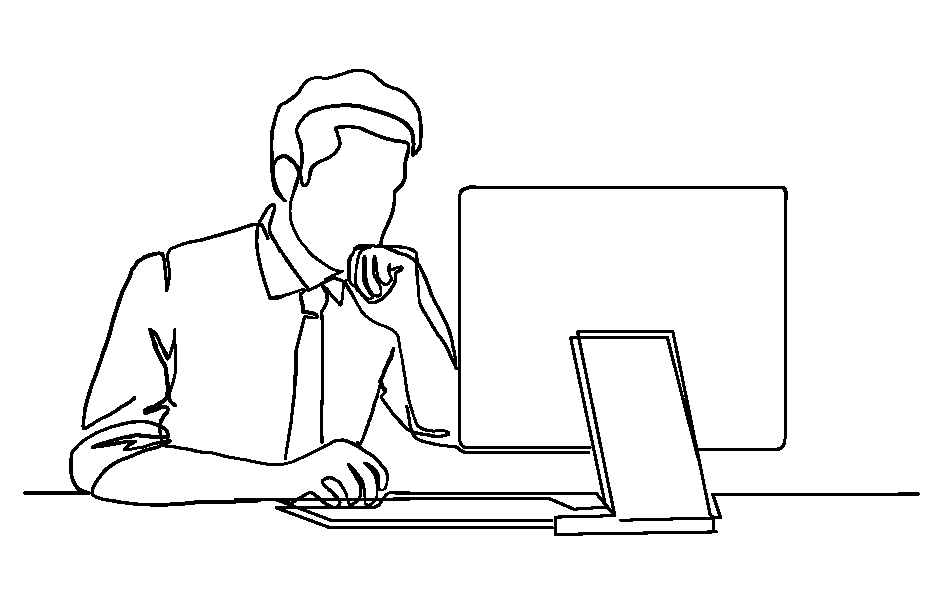
\includegraphics[width=0.55\textwidth]{files/drawing.pdf}
    \fbox{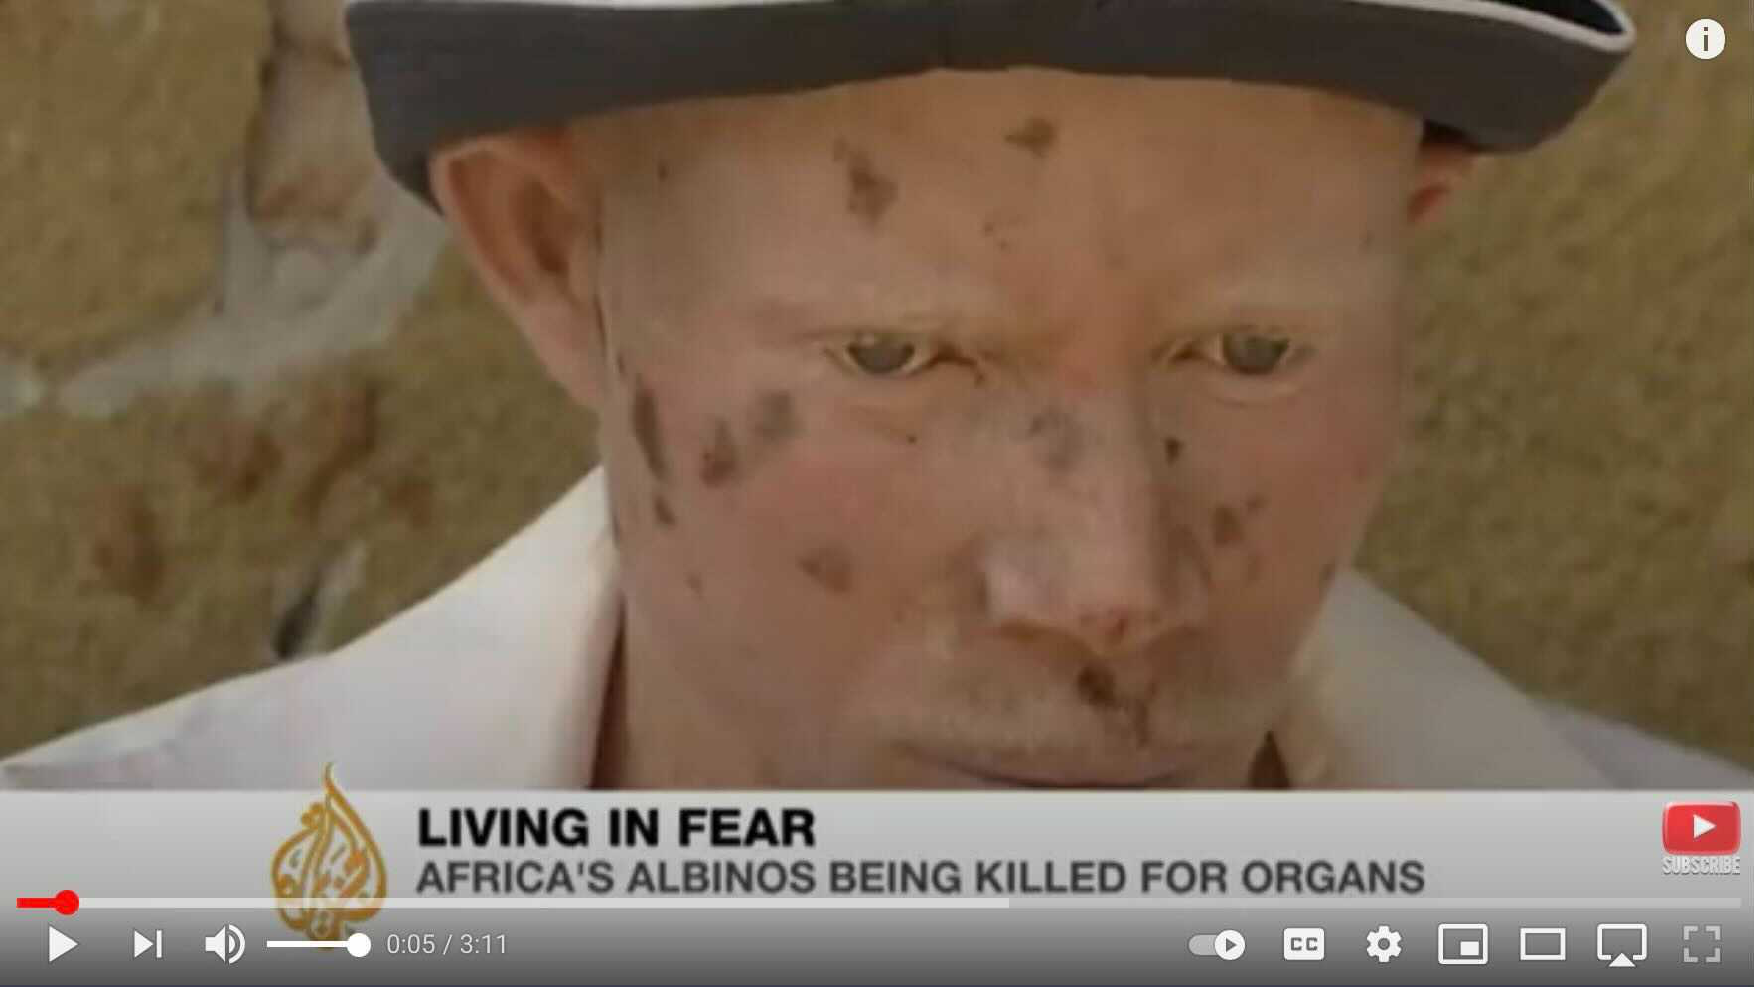
\includegraphics[width=0.35\textwidth]{files/video-snapshot.pdf}}\\[0.5em]
    \hspace{7.7cm} \footnotesize Figure 1: Snapshot of YouTube video
\end{figure}
\end{frame}

\begin{frame}{The Setting}
    \vspace{-1cm}
    \hspace{0.5cm}
    \begin{centering}
     \begin{tikzpicture}

         % time line
         \draw[line width=0.25mm, ->] (-3.75,0) -- (3.5,0) node [below] {};
         \draw (-3.25, -0.1) -- (-3.25, 0.1) node [below] {\shortstack{\\ \footnotesize Video Start}};
         \draw (2.5, -0.1) -- (2.5, 0.1) node [below] {\shortstack{\\ \footnotesize Video End}};

         % horizontal scale
         \draw[line width=0.25mm] (7, -3) -- (7, 3) node [above] {Sentiment};
         \foreach \x in {-3,-2,...,3}
            \draw (6.8, \x) -- (7.2, \x);

         \node[align=right] at (7.5, 0) {$0$};
         \draw[color=bonnblue, line width=0.3mm] (6.8, 1) -- (7.2, 1);

         % time-point
         \draw[line width=0.3mm, color=bonnblue] (-1, 0.1) -- (-1, -0.1);
         \node[] at (-1, -0.75) {\textcolor{bonnblue}{$\bm{t}$}};
         \draw[color=bonnblue, line width=0.3mm, ->] (-1, 0.25) .. controls (1, 1) and
             (3, 3) .. (5.5, 1) node [right] {\textcolor{bonnblue}{$\bm{X_i(t)}$}};

         \pause
         
         % outcome
         \draw[color=bonngrey, line width=0.3mm, ->] (2.5, -0.5) .. controls (2, -2) and (1.25, -2.2) .. (0, -2.5) node [left] {\textcolor{bonngrey}{$\bm{Y_i} \in \{0, 1\}$}};
         
     \end{tikzpicture}
 \end{centering}
\end{frame}


\newcommand{\brownianmotion}[5]{% points, advance, rand factor, options, end label
\draw[#4] (0,0)
\foreach \x in {1,...,#1}
{   -- ++(#2,rand*#3)
}
node[right] {#5};
}

\begin{frame}{The Data}{Regressors}
\pgfmathsetseed{1341}
\begin{centering}
\begin{tikzpicture}
    \draw[line width=0.25mm, ->] (0, -2) -- (0, 3);
    \draw[line width=0.25mm, ->] (-1, 0) -- (11, 0) node [below] {$t$};
    \brownianmotion{180}{0.05}{0.25}{color=bonngrey, line width=0.2mm}{$X_3(t)$}
    \brownianmotion{180}{0.05}{0.25}{color=bonnyellow, line width=0.2mm}{$X_2(t)$}
    \brownianmotion{180}{0.05}{0.25}{color=bonnblue, line width=0.2mm}{$X_1(t)$}
\end{tikzpicture}
\end{centering}
\end{frame}


\begin{frame}{The Problem}
\pgfmathsetseed{1341}
\vspace{-1cm}
\begin{tikzpicture}[scale=0.8]

    \draw[line width=0.25mm, ->] (0, -2) -- (0, 3);
    \draw[line width=0.25mm, ->] (-1, 0) -- (11, 0) node [below] {$t$};
    \brownianmotion{180}{0.05}{0.25}{color=bonngrey, line width=0.2mm}{$X_3(t)$}
    \brownianmotion{180}{0.05}{0.25}{color=bonnyellow, line width=0.2mm}{$X_2(t)$}
    \brownianmotion{180}{0.05}{0.25}{color=bonnblue, line width=0.2mm}{$X_1(t)$}

    \node[] at (12, 4) {$Y_1 \simeq g\big(X_1(\tau_1), X_1(\tau_2)\big)$};

    \draw[line width=0.2mm, dashed] (2, 4) -- (2, -3) node [right] {$\tau_1$};
    \draw[line width=0.2mm, dashed] (5, 4) -- (5, -3) node [right] {$\tau_2$};

    \node[circle, draw=black, minimum size=1mm, scale=0.9] (c1) at (2, 1.9) {};
    \draw[line width=0.2mm, ->] (c1) .. controls (3, 6) and (10, 6) .. (11.5, 4.5);

    \node[circle, draw=black, minimum size=1mm, scale=0.9] (c2) at (5, 2.6) {};
    \draw[line width=0.2mm, ->] (c2) .. controls (10, 2) and (12.5, 2.5) .. (13, 3.6);

\end{tikzpicture}
\end{frame}


\subsection{The Model}

\begin{frame}{The Model}

    \vspace{-1cm}
    \begin{align*}
        \tcbhighmath[fuzzy halo=1mm with bonnblue,arc=2pt, boxrule=0pt,frame
        hidden]{
            Y_i = g\left(X_i(\tau_1), \dots, X_i(\tau_S) \right) +  \epsilon_i
        }
    \end{align*}

    \vspace{0.5cm}
    \begin{table}[]
    \renewcommand{\arraystretch}{1.5}
        \begin{tabular}{ll}
          \labelitem $X_i = \{ X_i(t) : t \in [0, 1]\}$ & square integrable process\\
          \labelitem $\mathbb{E}\left[\epsilon_i \mid X_i(t) \right] = 0$ &  exogeneity\\
          \labelitem $g : \mathbb{R}^S \to \mathbb{R}$ & \emph{unknown} link function \\
          \labelitem $\tau_1, \dots, \tau_S \in [0, 1]$ &  \emph{unknown} points of impact
        \end{tabular}
    \end{table}

\end{frame}


\begin{frame}{Approach}

    \begin{table}[]
    \renewcommand{\arraystretch}{1.5}
        \begin{tabular}{ll}

        \textcolor{bonnblue}{$1$. stage} & Estimate $S$ and $\tau_1, \dots, \tau_S$\\
        \textcolor{bonnblue}{$2$. stage} & Estimate link function $g$

        \end{tabular}
    \end{table}

    \vspace{1cm}
    \emph{Focus here:} 1. stage

\end{frame}

\section{The Model}


\begin{frame}{The Model}

    \vspace{-1cm}
    \begin{align*}
        \tcbhighmath[fuzzy halo=1mm with bonnblue,arc=2pt, boxrule=0pt,frame
        hidden]{
            Y_i = g\left(X_i(\tau_1), \dots, X_i(\tau_S) \right) +  \epsilon_i
        }
    \end{align*}

    \vspace{0.5cm}
    \begin{table}[]
    \renewcommand{\arraystretch}{1.5}
        \begin{tabular}{ll}
          \labelitem $\quad X_i = \{ X_i(t) : t \in [0, 1]\}$ & square integrable process\\
          \labelitem $\quad \mathbb{E}\left[\epsilon_i \mid X_i(t) \right] = 0$ &  exogeneity\\
          \labelitem $\quad g : \mathbb{R}^S \to \mathbb{R}$ & \emph{unknown} link function \\
          \labelitem $\quad \tau_1, \dots, \tau_S \in [0, 1]$ &  \emph{unknown} points of impact
        \end{tabular}
    \end{table}

\end{frame}


\begin{frame}{Approach}

    \begin{table}[]
    \renewcommand{\arraystretch}{1.5}
        \begin{tabular}{ll}

            \textcolor{bonnblue}{$1$. stage} & Jointly estimate $S$ and $\tau_1, \dots,
            \tau_S$\\
            \textcolor{bonnblue}{$2$. stage} & Estimate link function $g$

        \end{tabular}
    \end{table}


    \vspace{1cm}
    \emph{Focus here:} 1st stage

\end{frame}


\begin{frame}

    \begin{center}
        \includegraphics[width=0.95\textwidth]{../../bld/figures/cross-covariance.png}
    \end{center}


\end{frame}

\section{Heuristics}


\begin{frame}{Plan}

    \vspace{-0.5cm}
    \begin{table}[]
    \renewcommand{\arraystretch}{1.5}
        \begin{tabular}{ll}
          \labelitem Simple linear model & $Y_i = \beta_0 + \sum_{s = 1}^S \beta_s X_i(\tau_s) + \epsilon_i$\\
          \labelitem Gaussian Process Regressors &  $X_i \sim \mathcal{GP}(0, \sigma)$\\
        \end{tabular}
    \end{table}

    \vspace{0.5cm}
    \begin{table}[]
    \renewcommand{\arraystretch}{1.5}
        \begin{tabular}{ll}
            \blue{Task:} & Think of how to identify/estimate $\tau_s$ for different $\sigma$\\
            \grey{Kernels:} & White, Brownian Motion, Matern, RBF\\
            \yellow{First insight:} & Investigate object $\expectation{Y_i X_i(t)}$
        \end{tabular}
    \end{table}

\end{frame}


\begin{frame}{Building Intuition}

    What is the connection between the kernel and a sample trajectory?\\[2em]

    $\implies$ Visualization

\end{frame}


\begin{frame}{General Representation}

    \vspace{-0.5cm}
    \begin{align*}
    \label{eq:1}
    f_{XY}(t) &\stackrel{def}{=} \expectation{Y_i X_i(t)}\\
              &= \expectation{\left(\beta_0 + \sum_{s = 1}^S \beta_s X_i(\tau_s) + \epsilon_i\right) X_i(t)}\\
              &= \sum_{s = 1}^S \beta_s \, \expectation{X_i(\tau_s) X_i(t)}\\
              &= \sum_{s = 1}^S \beta_s \, \sigma(t, \tau_s)
    \end{align*}

\end{frame}


\begin{frame}{White Kernel}

\vspace{-1.2cm}
\begin{centering}
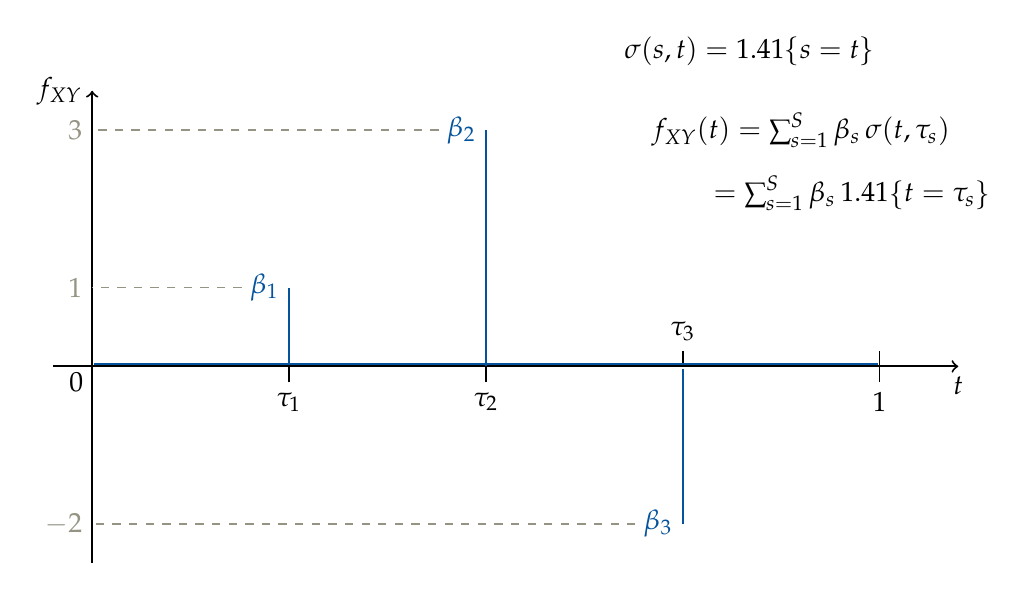
\begin{tikzpicture}

    \draw node at (8.35, 4) {$\sigma(s, t) = \indicator{s = t}$};
    \draw node at (9, 3) {$f_{XY}(t) = \sum_{s = 1}^S \beta_s \, \sigma(t, \tau_s)$};
    \draw node at (9.65, 2.2) {$= \sum_{s = 1}^S \beta_s \, \indicator{t = \tau_s}$};

    \draw[line width=0.25mm, ->] (0, -2.5) -- (0, 3.5) node [left] {$f_{XY}$};
    \draw[line width=0.25mm, ->] (-0.5, 0) -- (11, 0) node [below] {$t$};

    \draw (10, -0.2) -- (10, 0.2) node [below=0.4cm] {$1$};
    \draw node at (-0.2, -0.2) {$0$};

    \draw[line width=0.25mm] (2.5, -0.2) -- (2.5, 0) node [below=0.2cm] {$\tau_1$};
    \draw[line width=0.25mm] (5, -0.2) -- (5, 0) node [below=0.2cm] {$\tau_2$};
    \draw[line width=0.25mm] (7.5, 0) -- (7.5, 0.2) node [above] {$\tau_3$};

    \draw[line width=0.25mm, color=bonnblue] (0.02, 0.03) -- (9.98, 0.03) {};

    \draw[line width=0.25mm, color=bonnblue] (2.5, 0.03) -- (2.5, 1) node [left] {$\beta_1$};
    \draw[line width=0.25mm, color=bonnblue] (5, 0) -- (5, 3) node [left] {$\beta_2$};
    \draw[line width=0.25mm, color=bonnblue] (7.5, -0.03) -- (7.5, -2) node [left] {$\beta_3$};

    \draw[line width=0.2mm, color=bonngrey, dashed] (1.9, 1) -- (0, 1) node [left] {$1$};
    \draw[line width=0.2mm, color=bonngrey, dashed] (4.4, 3) -- (0, 3) node [left] {$3$};
    \draw[line width=0.2mm, color=bonngrey, dashed] (6.9, -2) -- (0, -2) node [left] {$-2$};

\end{tikzpicture}
\end{centering}
    
\end{frame}


\begin{frame}{Brownian Motion}

\vspace{-1.2cm}
\begin{centering}
\begin{tikzpicture}

    \draw node at (8.35, 4) {$\sigma(s, t) = \min\{s, t\}$};
    \draw node at (9, 3) {$f_{XY}(t) = \sum_{s = 1}^S \beta_s \, \sigma(t, \tau_s)$};
    \draw node at (9.65, 2.2) {$= \sum_{s = 1}^S \beta_s \, \min\{t, \tau_s\}$};

    \draw[line width=0.25mm, ->] (0, -2.5) -- (0, 3.5) node [left] {$f_{XY}$};
    \draw[line width=0.25mm, ->] (-0.5, 0) -- (11, 0) node [below] {$t$};

    \draw (10, -0.2) -- (10, 0.2) node [below=0.4cm] {$1$};
    \draw node at (-0.2, -0.2) {$0$};

    \draw[line width=0.25mm] (2.5, -0.2) -- (2.5, 0) node [below=0.2cm] {$\tau_1$};
    \draw[line width=0.25mm] (5, -0.2) -- (5, 0) node [below=0.2cm] {$\tau_2$};
    \draw[line width=0.25mm] (7.5, -0.2) -- (7.5, 0) node [below=0.2cm] {$\tau_3$};

    \draw[line width=0.25mm, dashed, color=bonngrey] (2.5, 0) -- (2.5, 1);
    \draw[line width=0.25mm, dashed, color=bonngrey] (5, 0) -- (5, 1.5);
    \draw[line width=0.25mm, dashed, color=bonngrey] (7.5,0) -- (7.5, 0.5);

    \draw[line width=0.25mm, color=bonnblue] (0.02, 0.03) -- (2.5, 1);
    \draw[line width=0.25mm, color=bonnblue] (2.5, 1) -- (5, 1.5);
    \draw[line width=0.25mm, color=bonnblue] (5, 1.5) -- (7.5, 0.5);
    \draw[line width=0.25mm, color=bonnblue] (7.5, 0.5) -- (10, 0.5);

\end{tikzpicture}
\end{centering}
    
\end{frame}


\begin{frame}

    \begin{center}
        \includegraphics[width=0.95\textwidth]{../../bld/figures/cross-covariance.png}
    \end{center}

\end{frame}


\begin{frame}{How do we find $\tau$?}

\begin{centering}
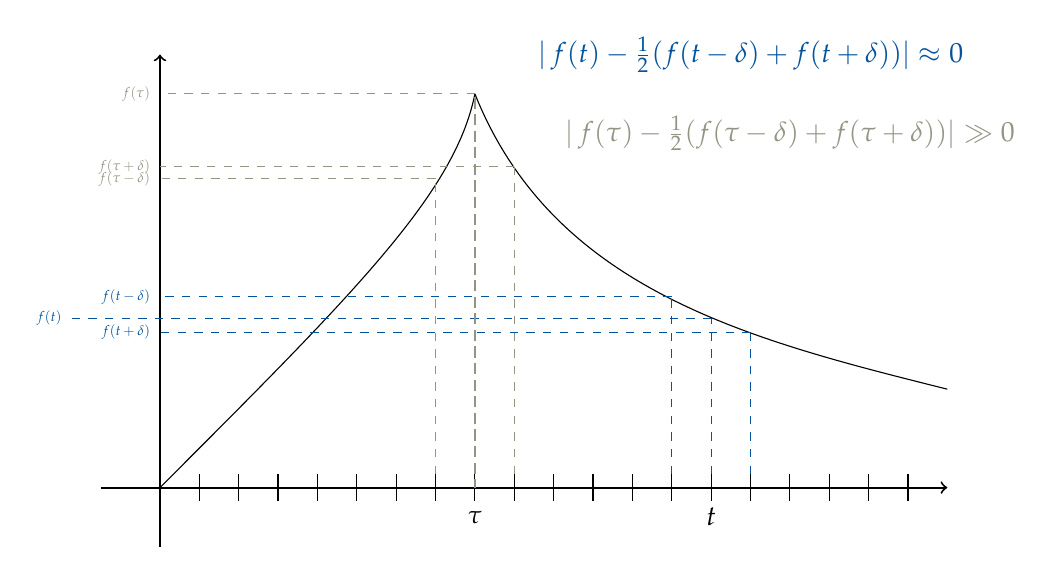
\begin{tikzpicture}[scale=2.5]
    \draw[line width=0.25mm, ->] (0, -0.3) -- (0, 2.2);
    \draw[line width=0.25mm, ->] (-0.3, 0) -- (4, 0);

    \draw (0, 0) .. controls (1, 1) and (1.5, 1.5) .. (0.2*8, 2);
    \draw (0.2*8, 2) .. controls (2, 1) and (3, 0.75) .. (4, 0.5);

    \draw[line width=0.2mm, dashed, color=bonngrey] (0.2*8, 0.07) -- (0.2*8, 2);
    \draw node at (0.2*8, -0.15) {\small $\tau$};

    \foreach \x in {1,...,19}
        \draw[thin] (0.2*\x, 0.07) -- (0.2*\x, -0.07);

    \draw[thin, dashed, color=bonnblue] (0.2*13, 0.07) -- (0.2*13, 0.97);
    \draw[thin, dashed, color=bonnblue] (0.2*14, 0.07) -- (0.2*14, 0.86);
    \draw[thin, dashed, color=bonnblue] (0.2*15, 0.07) -- (0.2*15, 0.79);
    \draw node at (0.2*14, -0.15) {$t$};

    \draw[thin, dashed, color=bonnblue] (0.2*13, 0.97) -- (0, 0.97) node [left] {\tiny
        $f(t - \delta)$};
    \draw[thin, dashed, color=bonnblue] (0.2*14, 0.86) -- (-0.45, 0.86) node [left] {\tiny
        $f(t)$};
    \draw[thin, dashed, color=bonnblue] (0.2*15, 0.79) -- (0, 0.79) node [left] {\tiny
        $f(t + \delta)$};

    \draw node at (3, 2.2) {\blue{$|\,f(t) - \frac{1}{2} (f(t - \delta) + f(t + \delta))| \approx
        0$}};

    \draw[thin, dashed, color=bonngrey] (0.2*7, 0.07) -- (0.2*7, 1.57);
    \draw[line width=0.2mm, dashed, color=bonngrey] (0.2*8, 0) -- (0.2*8, 2);
    \draw[thin, dashed, color=bonngrey] (0.2*9, 0.07) -- (0.2*9, 1.63);
    
    \draw[thin, dashed, color=bonngrey] (0.2*7, 1.57) -- (0, 1.57) node [left] {\tiny
        $f(\tau - \delta)$};
    \draw[thin, dashed, color=bonngrey] (0.2*8, 2)   -- (0, 2) node [left] {\tiny
        $f(\tau)$};
    \draw[thin, dashed, color=bonngrey] (0.2*9, 1.63)-- (0, 1.63) node [left] {\tiny
        $f(\tau + \delta)$};

    \draw node at (3.2, 1.8) {\grey{$|\,f(\tau) - \frac{1}{2} (f(\tau - \delta) + f(\tau +
    \delta))| \gg 0$}};


\end{tikzpicture}
\end{centering}

\end{frame}


% \begin{frame}{Finite Difference and Differentiability}
%     \vspace{-1cm}
%     Let $h: [0, 1] \to \mathbb{R}$.
% 
%     \vspace{0.25cm}
%     \blue{Definition.}\\
%         \quad $h$ is differentiable at $t \in (0, 1)$ if
%         $\lim_{\delta \to 0} (h(t + \delta) - h(t - \delta)) / \delta$ exists.
% 
%     \vspace{0.5cm}
%     \blue{Definition.}\\
%         \quad $C = C(t, \delta; h) = h(t + \delta) - h(t - \delta)$ is the (first-order)
%         centered difference of $h$.\\
%         \quad For small $\delta$, $h'(t)$ is approximated by $C / \delta$.
% 
%     \vspace{0.5cm}
%     \blue{Second derivative.}\\
%         \quad Applying the first-order centered difference twice yields the second-order\\
%         \quad difference $C^2 = C^2(t, \delta; h) = h(t + \delta) + h(t - \delta) -
%         2h(t)$. For small $\delta$, $h''(t)$ is\\ \quad approximated by $C^2 / \delta$.
% 
% \end{frame}


% \begin{frame}{Connecting Ideas}
% 
%     \begin{itemize}
%     \setlength\itemsep{1.5em}
%         \item[\labelitem] $f_{XY}(t) - \frac{1}{2}\left(f_{XY}(t + \delta) + f_{XY}(t -
%             \delta)\right) $ \pause
%         \item[\labelitem] $C^2(t, \delta; f_{XY}) = \left(f_{XY}(t + \delta) + f_{XY}(t
%             - \delta)\right) - 2 f_{XY}(t)$ \pause
%         \item[\labelitem] $\implies C^2(t, \delta; f_{XY}) = - 2 \Big[ f_{XY}(t) -
%                 \frac{1}{2} \left(f_{XY}(t + \delta) + f_{XY}(t - \delta)\right) \Big]$
%     \end{itemize}
% 
% \end{frame}


\begin{frame}{Estimation?}
    \begin{itemize}
    \setlength\itemsep{1.5em}
        \item[\labelitem] $Z_{\delta, i}(t) := X_i(t) - \left(X_i(t + \delta) + X_i(t -
            \delta)\right) / 2$
        \item[\labelitem] $\implies \expectation{Z_{\delta, i}(t) Y_i} = f_{XY}(t) -
            \frac{1}{2}\left(f_{XY}(t + \delta) + f_{XY}(t - \delta)\right)$
        \item[\labelitem] Estimate by: $\,\, n^{-1}\sum_{i=1}^n Z_{\delta, i}(t) Y_i$
        \item[\labelitem] Denote by: $f_{ZY}$ and $\hat{f}_{ZY}$
        \item[\labelitem] But what about $\delta$? \pause $\implies$ Visualization
    \end{itemize}
\end{frame}

\section{Identification}

\section{Estimation}

\section{Application}



\begin{frame}{References}
    \nocite{*}
    \printbibliography
\end{frame}

\setbeamertemplate{footline}[frame number]{}  % contact page has no frame number
\setbeamertemplate{navigation symbols}{}
\setbeamertemplate{footline}{}
\begin{frame}{Contact}
    \begin{itemize}
        \item[] \large \faIcon{github} \,\,\, \texttt{github.com/timmens/topics-metrics-2021}
        \item[] \large \faIcon{envelope} \,\, \texttt{tmensinger(at)uni-bonn.de}
    \end{itemize}
\end{frame}


\end{document}
